\documentclass[12pt]{article}
\usepackage[margin=2.5cm]{geometry}
\usepackage{enumerate}
\usepackage{amsfonts}
\usepackage{amsmath}
\usepackage{fancyhdr}
\usepackage{amsmath}
\usepackage{amssymb}
\usepackage{amsthm}
\usepackage{mdframed}
\usepackage{graphicx}
\usepackage{subcaption}
\usepackage{adjustbox}
\usepackage{listings}
\usepackage{xcolor}
\usepackage{booktabs}
\usepackage[utf]{kotex}

\definecolor{codegreen}{rgb}{0,0.6,0}
\definecolor{codegray}{rgb}{0.5,0.5,0.5}
\definecolor{codepurple}{rgb}{0.58,0,0.82}
\definecolor{backcolour}{rgb}{0.95,0.95,0.92}

\lstdefinestyle{mystyle}{
    backgroundcolor=\color{backcolour},
    commentstyle=\color{codegreen},
    keywordstyle=\color{magenta},
    numberstyle=\tiny\color{codegray},
    stringstyle=\color{codepurple},
    basicstyle=\ttfamily\footnotesize,
    breakatwhitespace=false,
    breaklines=true,
    captionpos=b,
    keepspaces=true,
    numbers=left,
    numbersep=5pt,
    showspaces=false,
    showstringspaces=false,
    showtabs=false,
    tabsize=1
}

\lstset{style=mystyle}

\begin{document}
\title{CSC148 Worksheet 14 Solution}
\author{Hyungmo Gu}
\maketitle

\section*{Question 1}
\begin{enumerate}[a.]
    \item

    \adjustbox{center,valign=t}{
        \begin{tabular}{|p{10cm}|c|}
            \hline
            \textbf{Operation} & \textbf{Running time}\\
            \hline
            Insert at the front of the list & $\mathcal{O}(n)$\\
            \hline
            Insert at the end of the list & $\mathcal{O}(1)$\\
            \hline
            Look up the element at index $i$, where $0 \leq i < n$ & $\mathcal{O}(n)$\\
            \hline
        \end{tabular}
    }

    \bigskip

    \begin{mdframed}
        \underline{\textbf{Correct Solution:}}

        \bigskip

        \adjustbox{center,valign=t}{
        \begin{tabular}{|p{10cm}|c|}
            \hline
            \textbf{Operation} & \textbf{Running time}\\
            \hline
            Insert at the front of the list & $\mathcal{O}(n)$\\
            \hline
            Insert at the end of the list & $\mathcal{O}(1)$\\
            \hline
            Look up the element at index $i$, where $0 \leq i < n$ & $\color{red}\mathcal{O}(1)$\\
            \hline
        \end{tabular}
    }

    \end{mdframed}

    \item

    The inserting of an element at position $i$ requires $n - i$ elements to
    be shifted to right.

    \bigskip

    Using this fact, we can write the Big-Oh expression for inserting an item at
    index $i$ is $\mathcal{O}(n - i)$.
\end{enumerate}

\section*{Question 2}
\begin{enumerate}[a.]
    \item

    \bigskip

    \adjustbox{center,valign=t}{
        \begin{tabular}{|p{10cm}|c|}
            \hline
            \textbf{Operation} & \textbf{Running time}\\
            \hline
            Insert at the front of the linked list & $\mathcal{O}(1)$\\
            \hline
            Insert at the end of the linked list & $\mathcal{O}(n)$\\
            \hline
            Look up the element at index $i$, where $0 \leq i < n$ & $\mathcal{O}(n)$\\
            \hline
        \end{tabular}
    }

    \newpage

    \begin{mdframed}
        \underline{\textbf{Correct Solution:}}

        \bigskip

        \adjustbox{center,valign=t}{
            \begin{tabular}{|p{10cm}|c|}
                \hline
                \textbf{Operation} & \textbf{Running time}\\
                \hline
                Insert at the front of the linked list & $\mathcal{O}(1)$\\
                \hline
                Insert at the end of the linked list & $\mathcal{O}(n)$\\
                \hline
                Look up the element at index $i$, where $0 \leq i < n$ & $\color{red}\mathcal{O}(i)$\\
                \hline
            \end{tabular}
        }

    \end{mdframed}

    \item

    Without the traversal, the running time of inserting is $\mathcal{O}(1)$.

    \bigskip

    With the traversal, the running time of inserting is $\mathcal{O}(i)$.

\end{enumerate}

\section*{Question 3}
\begin{itemize}
    \item

    Unlike linked lists that store node at different memory location, array-based
    lists store elements in memory immediately one after another.

    \bigskip

    Assuming it's easier for memory to find and perform operations on elements
    located right after another, I believe it's significantly faster for
    array-based lists to insert an element at position $i$.

    \bigskip

    \begin{mdframed}
        \underline{\textbf{Correct Solution:}}

        \bigskip

        \color{red}
        Since $n - i = 1,000,000 - 500,000 = 500,000$, we can write
        $\mathcal{O}(n-i) \approx \mathcal{O}(i)$

        \bigskip

        Using this fact, we can conclude the speed of linked lists and array-based
        lists are roughly about the same.
        \color{black}
    \end{mdframed}

    \bigskip

    \underline{\textbf{Notes:}}

    \bigskip

    \begin{itemize}
        \item Noticed that professor compared the performance of linked lists
        and array-based list in terms of Big-Oh.
    \end{itemize}

\end{itemize}

\section*{Question 4}
\begin{enumerate}[a.]
    \item

    When $n = 1$, the total number of nodes traversed is 0. This is because
    we are only replacing None in \textit{self.\_first} with \textit{\_Node(item)}.

    \bigskip

    When $n = 2$, the total number of nodes traversed is 0. This is because after
    adding the first element, we start at \textit{self.\_first}, and add \textit{\_Node(item)}
    to \textit{self.\_first.next}.

    \bigskip

    When $n > 2$, the number of nodes traversed increases by 1 per item added starting
    with the $3^{rd}$ element, and this continues until $n - 1$ (where it
    represents the last item in a list). So in this case, the total number of nodes
    traversed is

    \begin{align}
        \sum\limits_{i=2}^{n-1} (i-1) &= \sum\limits_{i'= 1}^{n-2} i'\\
        &= \frac{(n-2)(n-1)}{2}
    \end{align}

    \bigskip

    \begin{mdframed}

        \bigskip

        \underline{\textbf{Correct Solution:}}

        \bigskip

        \color{red}The code for \textit{append} method tells us\color{black}

        \begin{lstlisting}[language=python,caption={linked\_list.py}]
        class LinkedList:
            ...
            def append(self, item: Any) -> None:
                """Append <item> to the end of this list.
                """
                if self._first is None:
                    self._first = _Node(item)
                else:
                    curr = self._first
                    while curr.next is not None:
                        curr = curr.next
                    curr.next = _Node(item)
        \end{lstlisting}

        \bigskip

        When $n = 1$, the total number of nodes traversed is 0. This is because
        we are only replacing None in \textit{self.\_first} with \textit{\_Node(item)}.

        \bigskip

        When \color{red}$n > 1$, we know the number of nodes traversal
        required to add an item increases by 1 starting with the $2^{nd}$
        element\color{black}\:and this continues until $n - 1$ (where it represents
        the last item in a list). So in this case, the total number of nodes traversed is

        \begin{align}
            \sum\limits_{i=1}^{n-1} i &= \frac{n(n-1)}{2}
        \end{align}
    \end{mdframed}

    \bigskip

    \underline{\textbf{Notes:}}

    \bigskip

    \begin{itemize}
        \item I am feeling blue. I feel csc 148 worksheets are designed
        to be used in class, with details and expectations to questions
        learned as students are interacting with professor.

        \item Learned that the number of node traversed means the
        number of nodes that needs to be traveled to get to the closest None.

        \bigskip

        \adjustbox{valign=t}{
            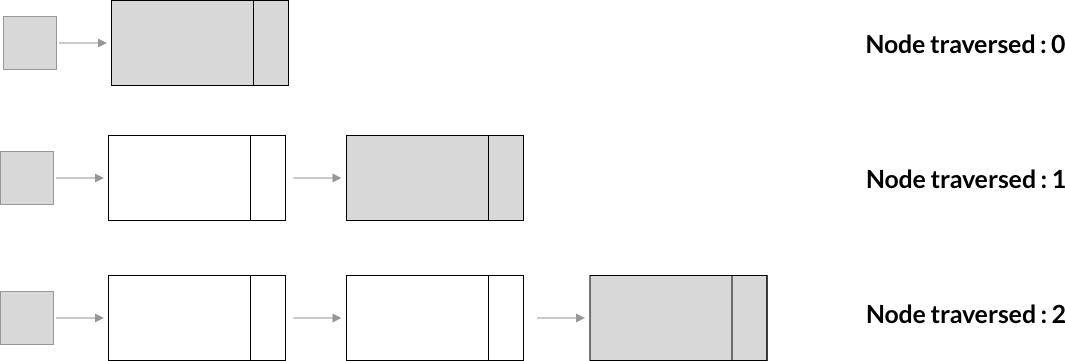
\includegraphics[width=\linewidth]{images/worksheet_14_q4a_notes.png}
        }
    \end{itemize}

    \item

    Since we know from previous problem that the running time of this operation
    is $\frac{n(n-1)}{2}$, we can conclude its Big-Oh expression is $\mathcal{O}(n^2)$.

\end{enumerate}

\section*{Question 5}
\begin{enumerate}[a.]
    \item It would be possible to return \textit{lst.\_\_contains\_\_(148)}
    after visiting just a single node if the first node of the linked list contains
    value 148.
    \item It would be necessary to visit all nodes in the linked list when
    no nodes contain value 148.
\end{enumerate}

\end{document}